%!TEX root = ../main.tex
\chapter{Implementación}
\label{chap:Implementación de la Ontologia}


La intención del trabajo es enriquecer los datos publicados por la DNCP en formato JSON a través de inserción de las propiedades necesarias para convertir un objeto JSON a JSON-LD para luego transformarlos a RDF. Una vez construida la base de datos en formato RDF se podrá montar a un punto SPARQL para realizar consultas y experimentaciones.


\begin{figure}[h!]
   \centering
   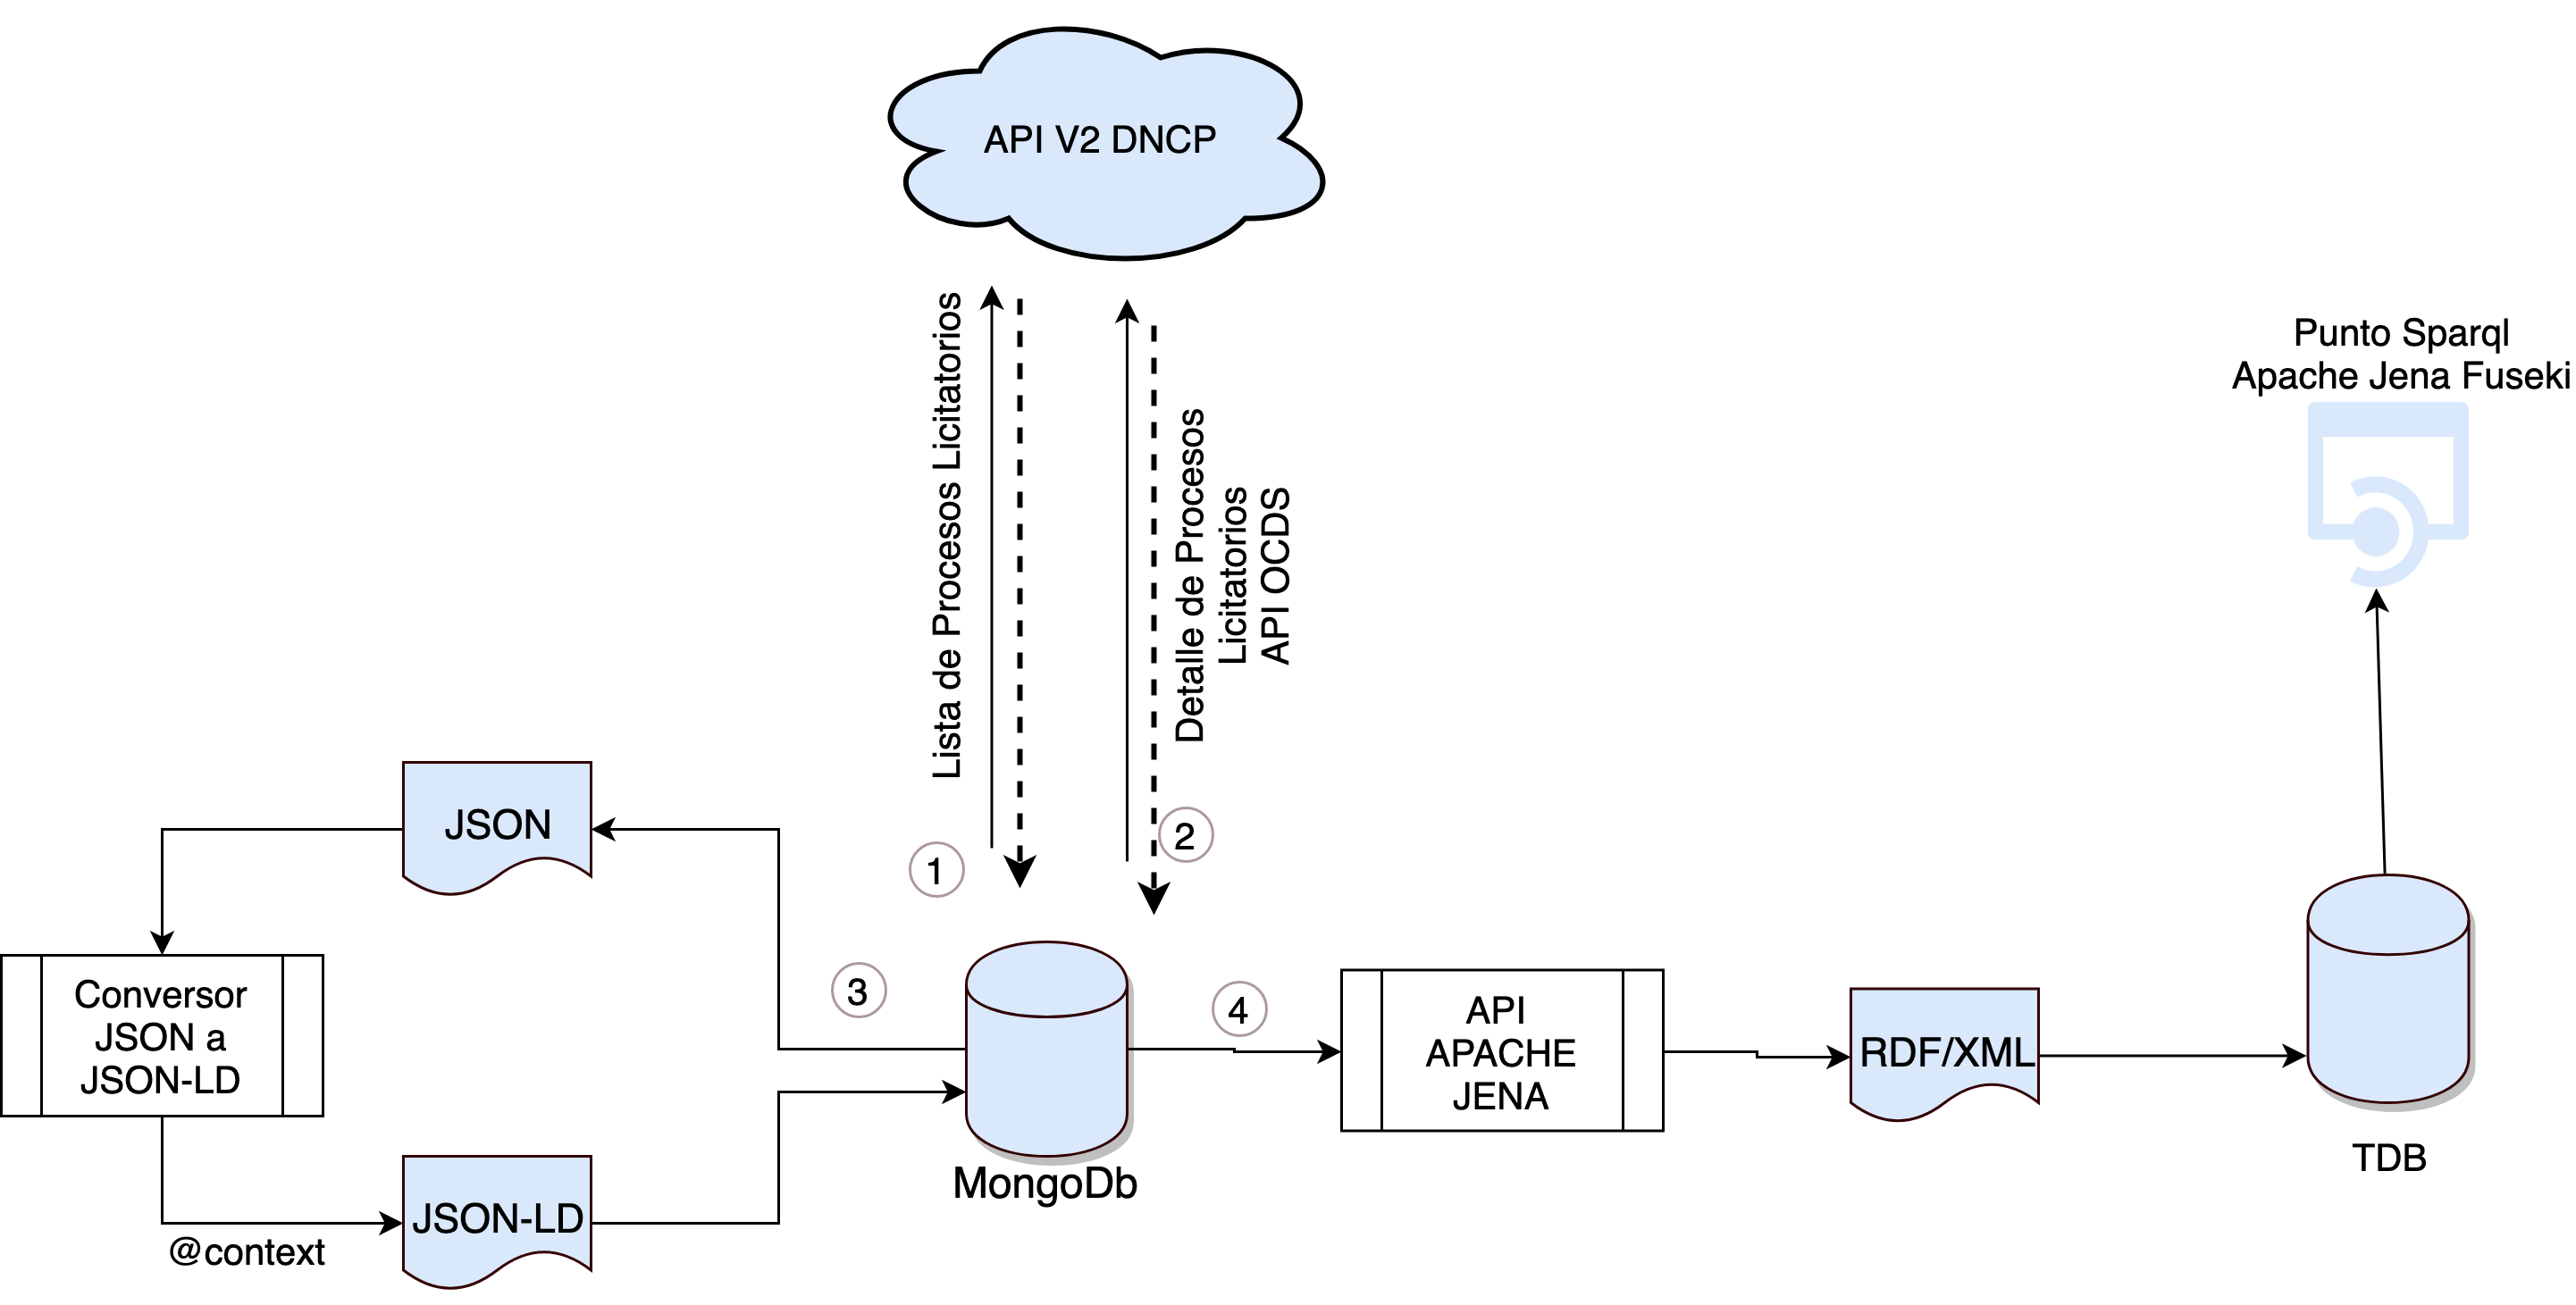
\includegraphics[width=150mm]{figuras/Diagramas-Implementacion.png}

   \caption{Modelo de Implementación}
   \label{img:modelo de Implementacion}
\end{figure}

A continuación explicaremos algunos conceptos relacionados y también las tareas realizadas para lograr montar correctamente el punto SPARQL.


\section{Contexto JSON-LD}

Como se vió anteriormente, existen varias formas de serialización de RDF, en contraste a XML, JSON-LD fue diseñado para ser un formato de intercambio de datos ligero e independiente del lenguaje y es lo suficientemente expresivo como para soportar los conceptos de RDF, además requiere poco esfuerzo para los desarrolladores transformar un documento JSON a JSON-LD\cite{JSONLDJS41:online}. 

Para dar contexto a un objeto JSON es necesario agregar el atributo @context. Éste puede darse de dos formas, definiendo la estructura del contexto como valor de la propiedad, o haciendo referencia (URI) a un documento que contiene la definición del contexto como ya se vió en la sección \ref{section:serializacion_jsonld}.

Se puede ir agregando @context a los objetos hijos de forma recursiva. Esto es muy importante debido a que se pueden sobrescribir los contextos exclusivamente para un objeto en particular sin que afecte a la definición de los demás. Más adelante en este capítulo se abordarán cada uno de los temas.



 
\section{De JSON a JSON-LD}
\label{section:jsonajsonld}

Se consultó la API de la DNCP que sigue el formato de OCDS, a modo de ejemplo se utlizó el proceso de licitación número 193399 a través de la siguiente URL https://www.contrataciones.gov.py/datos/api/v2/doc/ocds/record-package/193399.

Se extrajo solamente el objeto \textit{Compiled Release} (ver sección \ref{record}), que posee toda la información del proceso licitatorio. Una versión resumida del objeto se puede visualizar en el Cuadro \ref{lst:json1}. Se puede ver que el objeto tiene las siguientes propiedades: language, ocid, date, tag, initiationType, planning, tender, buyer, awards, contracts.\hfill \break

\noindent\begin{minipage}{\textwidth}
\begin{lstlisting}[captionpos=b, caption=Objeto JSON del OCDS de un Compiled Release, label=lst:json1,  numbers=left, language=json, numberstyle=\tiny\color{mygray},frame=single]
"compiledRelease": {
    "language": "es",
    "ocid": "ocds-03ad3f-193399",
    "id": "193399-adquisicion-scanner",
    "date": "2018-12-18T23:39:23Z",
    "tag": [
        "compiled"
    ],
    "initiationType": "tender",
    "planning": { ...
    },
    "tender": { ...
    },
    "buyer": { ...
    },
    "awards": [ ...
    ],
    "contracts": [ ...
    ]
}
\end{lstlisting}
\end{minipage}


Para enriquecer semánticamente un objeto debemos agregar un contexto y los respectivos @id para poder convertirlo a JSON-LD. 

Se encontró que no sería suficiente un solo contexto para todo el objeto. Esto se debe a las colisiones que existen entre propiedades que poseen el mismo nombre y distintos significados.

Dado que la definición de los contextos se da en forma de cascada, es decir se toma la definición más próxima, se definió un contexto para cada objeto hijo.

A continuación se muestra la colisión entre conceptos, donde \textit{amount} (del objeto \textit{budget}) se refiere al valor monetario (número y moneda) del presupuesto y la siguiente propiedad \textit{amount} (del objeto \textit{amount}) se refiere al valor numérico específicamente.\hfill \break

\noindent\begin{minipage}{\textwidth}
\begin{lstlisting}[captionpos=b, caption=Objeto JSON con colisión semántica entre conceptos, label=lst:oJson,language=json,firstnumber=1,  numbers=left,  numberstyle=\tiny\color{mygray},frame=single]
    "budget": {
        "description": "Adquisicion de Scanner",
        "amount": {
              "amount": 12000000,
              "currency": "PYG"
         }
     }  
    \end{lstlisting}
\end{minipage}
\noindent
\begin{minipage}{\textwidth}
    \begin{lstlisting}[captionpos=b, caption=Objeto JSON-LD sin colisión semántica entre conceptos , label=lst:oJsonLd, language=json,firstnumber=1,  numbers=left,  numberstyle=\tiny\color{mygray},frame=single]
    "budget": {
        "@context": "http://purl.org/onto-ocds/ocds/context-budget.json",
        "@type": "Budget",
        "description": "Adquisicion de Scanner",
        "amount": {
            "@context": "http://purl.org/onto-ocds/ocds/context-value.json",
            "@type": "Value",
            "amount": 12000000,
            "currency": "PYG"
       }
   }   
        \end{lstlisting}
    \end{minipage}

En el Cuadro \ref{lst:oJsonLd} se observa la solución implementada de manera a que el objeto \textit{budget} tenga la definición de su atributo \textit{amount} y el objeto \textit{amount} tenga la definición de su atributo \textit{amount} por separado evitando así inconsistencias.

Si bien las propiedades tienen el mismo nombre (o identificador) tienen definiciones distintas en cuanto a la sintaxis y a la semántica. En el caso de la propiedad de la línea 5 se refiere al valor monetario del presupuesto que está compuesto por la moneda y el valor numérico y está representado mediante un objeto JSON. En el caso de la propiedad de la línea 8 se refiere únicamente al valor numérico y está representado a través de un atributo de tipo numérico. 


A modo de ejemplo, se procedió a crear un contexto para el objeto planning que se muestra en el Cuadro \ref{lst:json2} y todos los objetos hijos del mismo. En el Cuadro \ref{lst:json3} se puede observar que se agregaron las propiedades @context en las líneas 2,6,10, la propiedad @type en las líneas 3,7,11 y la propiedad @id en la línea 4.

Se utilizó la herramienta JSON-LD PLAYGROUND \cite{JSONLDPl78:online} y RDF Translator\cite{RDFTrans0:online} para verificar la sintaxis de los documentos creados.\hfill \break

\noindent\begin{minipage}{\textwidth}
\begin{lstlisting}[captionpos=b, caption=Objeto JSON del OCDS de un Planning, label=lst:json2,  numbers=left, language=json, firstnumber=1, numberstyle=\tiny\color{mygray},frame=single]
"planning": {
    "budget": { 
        "description": "Adquisicion de Scanner",
        "amount": {
            "amount": 12000000,
            "currency": "PYG"
        }
    },
    "url": "https://www.contrataciones.gov.py/datos/id/planificaciones/193399-adquisicion-scanner"
}
\end{lstlisting}
\end{minipage}

\hfill \break

\noindent\begin{minipage}{\textwidth}
\begin{lstlisting}[captionpos=b, caption=Objeto JSON-LD del OCDS de un Planning, label=lst:json3,  numbers=left, language=json, firstnumber=1, numberstyle=\tiny\color{mygray},frame=single]
"planning": {
    "@context": "http://example.com/ocds/context-planning.json",
    "@type": "Planning",
    "@id": "https://www.contrataciones.gov.py/datos/id/planificaciones/193399-adquisicion-scanner"
    "budget": { 
        "@context": "http://example.com/ocds/context-budget.json",
    "@type": "Budget",
        "description": "Adquisicion de Scanner",
        "amount": {
            "@context": "http://example.com/ocds/context-value.json",
            "@type": "Value",
            "amount": 12000000,
            "currency": "PYG"
        }
    },
    "url": "https://www.contrataciones.gov.py/datos/id/planificaciones/193399-adquisicion-scanner"
}
\end{lstlisting}
\end{minipage}

Los documentos de los contextos sirven para referenciar a cada propiedad con la ontología creada. En el Cuadro \ref{lst:json4} se muestra el contenido del documento context-planning.json. Nótese de que sólo están definidas las propiedades hijas del objeto \textit{planning}, los demás ancestros se encuentran definidas en el documento del padre.

Además sólo se agregó la propiedad @id al objeto \textit{planning}, el objeto \textit{amount} no posee un @id debido a que la implementación de la DNCP tampoco provee un identificador único para ese objeto, esto significa que a conversión a RDF de dicho objeto derivará en un Blank Node, por lo que no será posible referenciar dicha instancia más allá de este documento. Eso tampoco es una necesidad para el nivel de agregación que se requiere ya que no es necesario identificar individualmente el monto. El monto siempre estará referenciado a través del objeto \textit{planning}

\hfill \break

\noindent\begin{minipage}{\textwidth}
\begin{lstlisting}[captionpos=b, caption=Contexto del Objeto Planning, label=lst:json4,  numbers=left, language=json, firstnumber=1, numberstyle=\tiny\color{mygray},frame=single]
"@context": {
    "Planning": {
        "@id": "http://w3id.org/ocds/ns#Planning"
    },
    "budget": {
        "@id": "http://w3id.org/ocds/ns#budget"
        "@type": "@id"
    },
    "url": {
        "@id": "http://w3id.org/ocds/ns#planningUrl"
        "@type": "http://www.w3/org/2001/XMLSchema#anyURI"
    }
}

\end{lstlisting}
\end{minipage}

Un inconveniente al momento de generar los valores para los atributos del @id, es que los objetos no posean un valor válido, en este caso una URI que desreferencie dicho objetos. El procedimiento consiste en verificar que el objeto posea un atributo “uri” cuyo valor sea una URI, de no ser el caso se procede a verificar si posee los atributos “url” e “id” sucesivamente. En el caso de que posea estos atributos pero con valores inválidos, osea no sean una URI propiamente dicha, se crea una URI ficticia a fin de que tenga un @id con formato válido. Si un objeto no tiene un @id válido, entonces no podrá ser convertido luego a formato RDF.

Otra excepción fue el caso de los Codelist abiertos y cerrados. En cada caso se procedió a transformar el valor del atributo correspondiente, que en este caso era un String que no era una URI, a una URI que referencia a una instancia del respectivo CodeList. A modo de ejemplo se transformaron valores de los atributos de \textit{TenderStatus}, \textit{AwardStatus}, \textit{ContractStatus}, \textit{Classification Scheme} que referencian a las instancias que se encuentran en la ontología desarrollada. Los demás Codelist ya poseen las instancias respectivas dentro de la ontología desarrollada, pero la conversión de los mismos en los datos de la DNCP quedó como futuro trabajo.

Se realizó el mismo procedimiento con los demás objetos pertenecientes al JSON. Como futuro trabajo se podrá optimizar el tiempo de carga del documento JSON-LD agregando contextos sólo cuando exista una colisión semántica, de esta manera se ahorrarán líneas de datos innecesarias.

Como siguiente paso queda convertir de manera programática los objetos publicados en JSON a JSON-LD para su posterior serialización a RDF.


\section{De JSON-LD a RDF}

La conversión de JSON-LD a RDF es un proceso directo. El sujeto (en JSON-LD), que podría ser usado como objeto en otra tripla, es definido por la propiedad @id, todas las demás propiedades son convertidas en predicado del objeto RDF resultante. Finalmente, los valores literales son extraídos directamente de la propiedad o del valor @value de la propiedad (si lo tuviere). Una propiedad puede tener también definido el lenguaje (@language) y/o tipo de informacion (@type).

Por ejemplo en la Figura \ref{img:EjemploBaranJSONLD} se muestra un objeto JSON-LD, que posee un contexto definido dentro del mismo objeto, este contexto también podría estar definido dentro de un documento diferente y referenciado a través de una URI. Tomemos como ejemplo la propiedad foaf:name, la misma se convierte en predicado y el objeto toma el valor del literal “Benjamin Baran” definido en el idioma inglés según especifica @language.



\begin{figure}[h!]
    \centering
    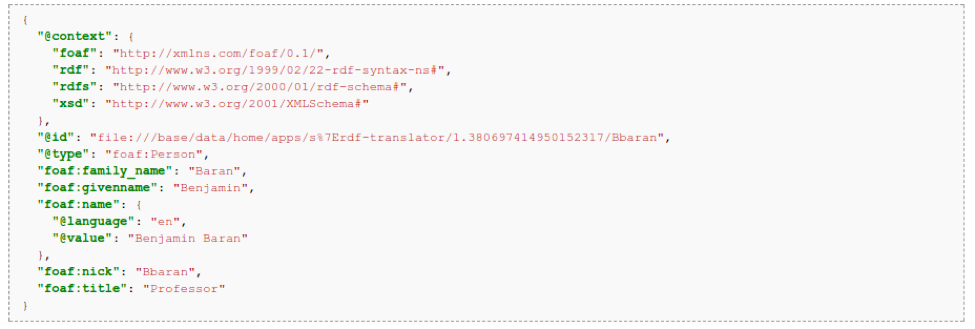
\includegraphics[width=150mm]{figuras/BaranJSONLD.png}
    \caption{Objeto JSON-LD}
    \label{img:EjemploBaranJSONLD}
    \end{figure}




\begin{figure}[h!]
    \centering
    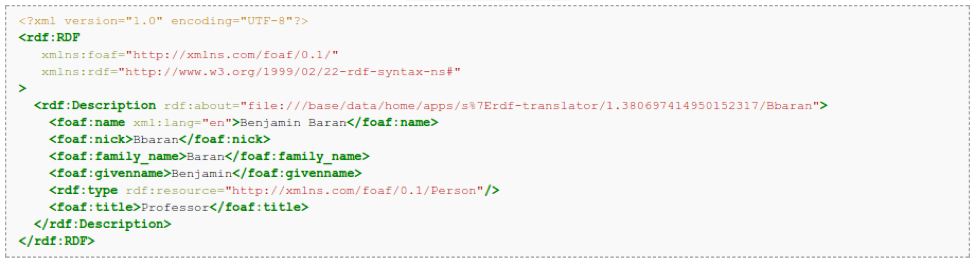
\includegraphics[width=150mm]{figuras/BaranRDF.png}
    \caption{Grafo RDF}
    \label{img:EjemploBaranRDF}
    \end{figure}




\section{Scrapper y convertidor de JSON-LD}

En la sección anterior se vio el proceso para convertir un objeto JSON a JSON-LD, esta sección se enfocará en automatizar el proceso de manera programática y tener una base de datos en formato RDF.

Como primer insumo se utilizó la API V2 de la DNCP, se utilizó como base un software desarrollado en Java por Diego Torres también para un trabajo de grado\footnote{https://github.com/diegotorrespy/scraper}, el mismo disponibilizó el trabajo bajo una licencia de libre uso. El software fue optimizado y adaptado según las necesidades de este trabajo, mejorando la velocidad de consulta de los registros y puesto de manera pública en un repositorio Git\footnote{https://github.com/camilobaezcamba/scraper}.


A continuación se desarrollarán los pasos seguidos que se indican en la Figura \ref{img:modelo de Implementacion}.

\textbf{Paso 1.} Se utilizó el servicio de buscador de contratos. Se utilizó el buscador para extraer los identificadores de los procesos licitatorios en un rango de fechas. Para este trabajo se decidió trabajar con contrataciones del 1 de Enero del 2016 al 31 de Diciembre del 2016, ya que los mismos contemplan un año completo de ejercicio fiscal y las variaciones de los contratos son mínimas con relación al año 2018.



\textbf{Paso 2.} Con los identificadores recogidos, se consultó la información del proceso licitatorio de la API que sigue los delineamientos de la OCDS. Al realizar las experimentaciones previas se detectó que el servicio tiende a fallar cuando se solicitan varios procesos licitatorios por segundo, por lo que el software hace varios intentos hasta conseguir descargar el registro. La cantidad y el intervalo entre cada intento es parametrizable dentro del software desarrollado.

El \textit{Record Package} contiene mucha información que todos los \textit{Releases} del proceso licitatorio. Para este trabajo se consideró solamente el \textit{Compiled Release} que se encuentra dentro del arreglo de \textit{Records}, el mismo contiene un recopilado de todos los \textit{Releases} y la versión final de todos los atributos. Con esta decisión, se pierde el historial de cambios que contempla el OCDS, aunque la DNCP tampoco implementó la publicación del historial de cambios.

El \textit{Compiled Release} es guardado en un sistema de base de datos no relacional, que nos permite guardar la información en formato JSON, se utilizó este sistema por su versatilidad para el manejo de documentos con este formato.

\textbf{Paso 3.} Luego de almacenar todos los procesos licitatorios en el sistema de base de datos (MongoDB), se realizó la conversión del objeto JSON a JSON-LD. Esto se hace sistemáticamente identificando las propiedades que son de tipo \textit{JsonObject} y agregando las propiedades @id, @context y @type según el nombre de la propiedad, siguiendo el procedimiento y las salvedades expuestas anteriormente (ver sección \ref{section:jsonajsonld}). Luego de la conversión se procede a guardar ese nuevo objeto JSON en una nueva colección en la base de datos mencionada.

\textbf{Paso 4.} El proceso siguiente fue la conversión de los objetos JSON-LD a RDF utilizando la librería Apache Jena. Una vez incluída la librería en el proyecto fue posible realizar esta conversión pasando los objetos JSON-LD e indicando la ubicación del TDB en la que se almacenarán los datos en RDF. TDB es una capa de almacenamiento de grafos.

De la misma manera se obtuvo los datos de todos los proveedores del Estado del servicio en JSON-LD que brinda la DNCP, se almacenó en la base de datos MongoDB para su posterior conversión a RDF. 

El software desarrollado\footnote{http://bit.ly/ValdezBaezThesis} va desde la obtención de los datos hasta la transformación y almacenamiento a RDF. Para este trabajo se optó por utilizar Apache Jena, por el gran soporte para JAVA, que es el lenguaje utilizado en el Scrapper de datos. Además cuenta con un servidor SPARQL llamado Apache Jena Fuseki.



\section{Punto SPARQL}
\label{section:puntosparql}

Para este trabajo se implementó el Punto SPARQL Jena Fuseki\cite{ApacheJe97:online} en un servidor para realizar las consultas. Cabe mencionar que todo lo desarrollado se hizo en un entorno experimental, como futuro trabajo queda hacer las optimizaciones correspondientes de tiempo de ejecución y uso de recursos para un entorno de producción o industrial.

Se consulta la colección de la base de datos MongoDB generada y se utiliza la librería JENA para transformar y convertir la serialización de JSON-LD a RDF. Luego de la serialización se procede a guardar los datos en un TDB, un sistema de almacenamiento y consulta de RDF, para que luego este sirva como insumo para el Punto SPARQL implementado utilizando Apache Jena FUSEKI en su versión 2.6.0.

Previo al despliegue del servidor fue necesario realizar una serie de configuraciones.

\begin{enumerate}
    \item Se indicaron los conjuntos de datos (TDB).
    \item Se configuraron dos servicios independientes (Procesos Licitatorios y Proveedores).
    \item Se activaron los servicios de razonamiento de FUSEKI indicando que utilizaremos las Reglas Básicas de Razonamiento de OWL. 
    \item Se realizó un ajuste a la cantidad máxima de memoria (RAM) utilizada. Se configuró en 4048 MB (-Xmx4048M) ya que la configurada por defecto ocasiona interrupciones o paradas inesperadas del servidor. Por defecto tiene definido como máximo 1200 MB (-Xmx1200M). Esta configuración se realizó en el script “fuseki-server” que se encuentra en la raíz del directorio de instalación y fue necesario modificar la variable “JVM\_ARGS” 

\end{enumerate}

La máquina en la cual se realizaron las pruebas tenía las prestaciones técnicas que se muestran en la Tabla \ref{tab:prestaciones_servidor}.


\begin{table}[!htb]
\centering
    \caption{Prestaciones del servidor utilizado para las pruebas}
    \label{tab:prestaciones_servidor}
\begin{tabular}{|l|l|}
\hline
 RAM & 16 GB\\\hline
    Disco duro & SSD 256\\\hline
    Sistema Operativo & macOS (Mojave), versión: 10.14.3\\\hline
    Procesador & Intel Core i7 2.6 GHz\\\hline
\end{tabular}
\end{table}


Una vez desplegado el servidor se procedió a cargar las ontologías correspondientes. Desde este momento el Punto SPARQL quedó totalmente configurado para realizar las consultas necesarias.

La Figura \ref{img:modelo de Implementacion} muestra el proceso de conversión, almacenamiento y disponibilización de datos.

\section{Conjuntos de datos para las pruebas de interoperabilidad}

Para probar el funcionamiento de la ontología creada se procedió al uso de una parte de la ontología implementada por la DNCP correspondiente a los proveedores del estado. Con el conjunto de datos de Proveedores podemos obtener datos adicionales sobre algún proveedor que se está presentando en algún proceso licitatorio.

Se utilizó para esto la API V2 de proveedores \footnote{\url{https://www.contrataciones.gov.py/datos/api/v2/doc/proveedores/}}, dicha API ya se encuentra publicada con el formato JSON-LD. Se realizaron consultas para obtener todos los registros de proveedores del estado y volcarlos a la base de datos MongoDB. Luego, utilizando la librería Jena, se procedió a convertir los objetos JSON-LD a RDF para posteriormente almacenarlos en la base de datos TDB.

Al momento de realizar las pruebas de interoperabilidad solamente se trabajó con un subconjunto (100) de los procesos licitatorios del año 2016. De esta manera se logró realizar consultas rápidas ya que se partió de una base de datos ligera y la intención fue probar la interoperabilidad semántica entre distintas fuentes de datos. Esto es meramente experimental y no fue una prioridad mejorar los tiempos de respuesta.

Como se había explicado anteriormente hemos utilizado los conjuntos de datos de Procesos Licitatorios y Proveedores para realizar consultas sobre el Punto SPARQL. A continuación expondremos algunos inconvenientes y las soluciones aplicadas referente a la manipulación de datos.

Para obtener los datos de la API V2 de la DNCP se procedió a registrarnos de manera a poder realizar peticiones sin limitaciones.

Al realizar la consulta a la API “Buscador de licitaciones” pasando como rango de fechas 01/01/2016 - 31/12/2016 se encontró que existen alrededor de 12.000 procesos licitatorios.
Dicho servicio retorna datos mínimos de cada proceso licitatorio de manera paginada, en este caso 1000. Luego, a partir del id de llamado (identificador único) se procedió a realizar las consultas al servicio de “Licitaciones” el cual está alineado al OCDS (estándar en el cual se basa la ontología desarrollada) para obtener los datos de manera más detallada.

En este proceso se identificaron varios inconvenientes en la comunicación con los servicios. El tiempo de respuesta se ve afectado por la cantidad de datos solicitados y por el intervalo de tiempo entre estas solicitudes de datos. Entonces se procedió a ajustar los parámetros de las peticiones, logrando conseguir un tiempo óptimo con las siguientes salvedades.

\begin{enumerate}

    \item Obtener los id de llamado (Buscador) de manera paginada (1000 registros).
    \item Cada 1000 registros obtenidos, lanzar 100 solicitudes paralelas de procesos licitatorios (Servicio OCDS) y esperar la respuesta de todas las peticiones para volver a realizar otras 100 solicitudes hasta completar el lote.
    \item A medida que se obtienen los procesos licitatorios se almacenan en la Base de datos MongoDB.
  
\end{enumerate}

La intención no fue optimizar el desempeño del software desarrollado sino lo necesario como para obtener los datos sin mayores inconvenientes y poder realizar todo el proceso de manera automatizada.










 \section{Discusión del Capítulo }

 Se puso a conocimiento los procesos realizados con relación a la manipulación de los datos así como también las cuestiones de implementación del software desarrollado y la utilización y configuración del Punto SPARQL (Jena Fuseki). Con todo esto puesto a punto, en la siguiente sección explicaremos el proceso de pruebas y resultados obtenidos.



